\documentclass{book}
\usepackage[a4paper]{geometry}
\usepackage[english]{babel}
\usepackage[utf8]{inputenc}
\usepackage{url}
\usepackage{hyperref}
\usepackage{float}
\usepackage{amsmath}
\usepackage{amsfonts}
\usepackage{amssymb}
\usepackage{amsthm}
\usepackage{eufrak}
\usepackage{algorithm}
\usepackage{algorithmicx}
\usepackage[noend]{algpseudocode}
\usepackage{xspace}
\usepackage{todonotes}

\theoremstyle{definition}
\newtheorem{defn}{Definition}
\theoremstyle{plain}
\newtheorem{lemma}{Lemma}
\newtheorem{theorem}{Theorem}

\DeclareMathOperator*{\argmax}{arg\,max}

\title{Documentation}
\author{Lucas Guesser Targino da Silva}

\begin{document}

\maketitle

\tableofcontents

\listoftodos

\newcommand{\R}{\mathbb{R}}
\newcommand{\N}{\mathbb{N}}
\newcommand{\Nb}[1]{\ensuremath{\N_{#1}}}
\newcommand{\Nt}{\Nb{2}}
\newcommand{\range}[1]{\ensuremath{\left[\left[ #1 \right]\right]}}
\newcommand{\Square}[1]{\ensuremath{sq({#1})}}
\newcommand{\tuple}[1]{\ensuremath{\left\langle #1 \right\rangle}}
\newcommand{\Set}[1]{\ensuremath{\left\{ #1 \right\}}}
\newcommand{\SetOf}[2]{\ensuremath{\Set{ #1 : #2}}}
\newcommand{\tupleOf}[2]{\ensuremath{\tuple{ #1 \ : \ #2}}}
\newcommand{\incl}[2]{#1 \triangleright #2}
\newcommand{\great}{Great\xspace}

\newcommand{\dref}[1]{Definition \ref{#1}\xspace}
\newcommand{\tref}[1]{Theorem \ref{#1}\xspace}

\newcommand{\op}{\ensuremath{\omega}}
\renewcommand{\b}[1]{\ensuremath{b\left( #1 \right)}}
\newcommand{\s}[1]{\ensuremath{s\left( #1 \right)}}
\newcommand{\price}[1]{\ensuremath{\rho\left( #1 \right)}}
\newcommand{\OS}{\ensuremath{\Omega_{n}}}
\newcommand{\pricep}[1]{\ensuremath{p_{\s{#1}} - p_{\b{#1}}}}

\newcommand{\sopt}{\ensuremath{S^{*}}}
\newcommand{\sop}{\ensuremath{\op^{*}}}

\chapter{Share Market}

\section{Basic Definitions}

\begin{defn}[Natural]
    Given $v \in \N$, we define:
    \begin{equation}
        \Nb{v} = \SetOf{n \in \N}{n \geqslant v}
    \end{equation}
\end{defn}

\begin{defn}[Range]
    \label{def:range}
    Given $n \in \Nt$, we define the \textbf{Range of $n$} as:
    \begin{equation}
        \range{n} = \Set{0, \dots, n - 1} = \SetOf{i \in \N}{i < n}
    \end{equation}
\end{defn}

\begin{defn}[Square]
    \label{def:square}
    Given $n \in \Nt$, we define the \textbf{Square of $n$} as:
    \begin{equation}
        \Square{n} = \range{n} \times \range{n}
    \end{equation}
\end{defn}

\section{Problem Definitions}

You are given an array in which the $i$th element is the price of a given stock on the day $i$. You are permitted to complete at most 1 transaction (i.e. buy once and sell once). What is the maximum profit you can gain?

Notice that you cannot sell a stock before buying it.

\subsection{Definitions}

\begin{defn}[Price Tuple]
    \label{def:price}
    Given $n \in \Nt$, a \textbf{Price Tuple} $p$ is a positive real tuple with $n$ elements:
    \begin{equation}
        p = \langle p_{0}, \dots, p_{n-1} \rangle \in \R^n_+
    \end{equation}
\end{defn}

\begin{defn}[Operation Pair]
    \label{def:op-pair}
    Given $n \in \Nt$, an \textbf{Operation Pair} $\op$ is a pair:
    \begin{equation}
        \op = \tuple{\b{\op}, \s{\op}} \in \Square{n}
        \quad ,
        b < s
    \end{equation}
    when the context is clear enough, we will simply write $\op = \tuple{\b{\op}, \s{\op}} = \tuple{b, s}$.
\end{defn}

\begin{defn}[Ascending Operation Pair]
    Given $n \in \Nt$ and a Price Tuple $p$, an Operation Pair $\op = \tuple{b, s}$ is said to be \textbf{Ascending} when:
    \begin{equation}
        p_{b} \leqslant p_{b+1} \leqslant \dots \leqslant p_{s-1} \leqslant p_{s}
    \end{equation}
\end{defn}

\begin{defn}[Maximal Operation Pair]
    \label{def:max-op-pair}
    Given $n \in \Nt$ and a Price Tuple $p$, we say that an Ascending Operation Pair $\op = \tuple{b, s}$ is a \textbf{Maximal Operation Pair}, or simply that $\op$ is \textbf{Maximal}, when it is Ascending and it satisfies the conditions:
    \begin{align}
        p_s - p_b \geqslant p_{s+1} - p_b \quad \mbox{, if } s+1 < n\\
        p_s - p_b \geqslant p_s - p_{b-1} \quad \mbox{, if } b-1 > 0
    \end{align}
\end{defn}

\begin{theorem}
    \label{theorem:max-op-pair}
    Given $n \in \Nt$ and a Price Tuple $p$, an Operation Pair $\op = \tuple{b, s}$ is Maximal if and only if the following conditions are satisfied:
    \begin{align}
        p_s \geqslant p_{s+1} \quad \mbox{, if } s+1 < n\\
        p_b \leqslant p_{b-1} \quad \mbox{, if } b-1 > 0
    \end{align}
\end{theorem}

\begin{proof}
    It comes directly from the inequalities of the \dref{def:max-op-pair}.
\end{proof}

\begin{defn}[Independent Operation Pairs]
    Given two Operation Pairs $\op, \op'$, we say that $\op, \op'$ are \textbf{Independent} when:
    \begin{equation}
        \s{\op} < \b{\op'} \lor \s{\op'} < \b{\op}
    \end{equation}
    moreover, given a set of Operation Pairs $S = \Set{\op_0, \dots, \op_{m-1}}$, we say that $S$ is independent when it satisfies:
    \begin{equation}
        \forall \op \forall \op' \left(
            \op \in S \land \op' \in S
            \rightarrow
            \op, \op' \mbox{ are independent}
        \right)
    \end{equation}
    i.e. all Operation Pairs $\op, \op' \in S$ are pairwise Independent.
\end{defn}

\begin{defn}[Operation Set]
    Given $n \in \Nt$, an \textbf{Operation Set} $S \subseteq \Square{n}$ is a set which satisfies:
    \begin{enumerate}
        \item $\forall \omega \left( \omega \in S \rightarrow \omega \mbox{ is an Operation Pair} \right)$
        \item $S$ is independent
    \end{enumerate}
    Moreover, we denote the set of all possible Operations Set by:
    \begin{equation}
        \OS = \SetOf{S \subseteq \Square{n}}{S \mbox{ is an Operation Set}}
    \end{equation}
\end{defn}

\begin{defn}
    Given an $n \in \Nt$, a Price Tuple $p$, and an Operation Set $S \in \OS$, the price $\price{S}$ of $S$ is:
    \begin{equation}
        \price{S} = \displaystyle\sum\limits_{\op \in S} p_{\s{\op}} - p_{\b{\op}}
    \end{equation}
\end{defn}

\begin{lemma}
    \label{lemma:opt-price-I}
    Given an $n \in \Nt$ and a Price Tuple $p$, if a Operation Set $\sopt \in \OS$ is has optimal price, then all Operation Pairs of $\sopt$ are Maximal, i.e.:
    \begin{align}
        \price{\sopt} = \max\limits_{S \in \OS} \left[ \price{S} \right]
        \rightarrow
        \forall \op \left( \op \in \sopt \rightarrow \op \mbox{ is Maximal} \right)
    \end{align}
\end{lemma}

\begin{proof}
    Suppose $\sopt \in \OS$ is a Operation Set with optimal price. Suppose by contradiction that $\exists \op \left( \op \in \sopt \land \op \mbox{ is not Maximal} \right)$, and let $\op = \tuple{b, s}$ be such Operation Pair. By \tref{theorem:max-op-pair}, one of the following cases must be true:
    \begin{enumerate}
        \item $p_s < p_{s+1} \quad \mbox{, if } s+1 < n$
        \item $p_b > p_{b-1} \quad \mbox{, if } b-1 > 0$
    \end{enumerate}

    \subsection*{Case 1} \label{proof:opt-price-I-case-1}
    Suppose that $p_s < p_{s+1}$, $s+1 < n$.
    
    \subsubsection*{Case 1.1}
    Suppose in addition that $\op' = \tuple{b, s+1}$ is independent of all $\op \in \sopt \backslash \Set{\op}$. Let $S' = (\sopt \backslash \Set{\op}) \cup \Set{\op'}$. Notice that 
    \begin{align}
        \price{\op} = \pricep{\op} < \pricep{\op'} = \price{\op'} 
    \end{align}
    Therefore $\price{\sopt} < \price{S'}$ (because $\sopt$ and $S'$ differ only in the elements above), contradicting the optimality of $\sopt$.
    
    \subsubsection*{Case 1.2}
    Suppose in addition that $\exists \op'(\op' \in \sopt \land \b{\op'} = s + 1)$, and let $\op' = \tuple{s+1, s'}$ be such Operation Pair. Let $\op'' = \tuple{b, s'}$ and $S'' = (\sopt \cup {\op''}) \backslash \Set{\op, \op'}$. Notice that
    \begin{align}
        \price{\op} + \price{\op'} & = \\\nonumber
        (\pricep{\op}) + (\pricep{\op'}) & = \\\nonumber
        (p_{s} - p_{b}) + (p_{s'} - p_{s+1}) & = \\\nonumber
        (p_{s'} - p_{b}) + (p_{s} - p_{s+1}) & < \\\nonumber
        p_{s'} - p_{b} & = \\\nonumber
        \price{\op''}
    \end{align}
    Therefore $\price{\sopt} < \price{S''}$ (because $\sopt$ and $S'$ differ only in the elements above), contradicting the optimality of $\sopt$.

    \subsubsection*{Case 1 - Conclusion}
    The hypothesis $p_s < p_{s+1}$, $s+1 < n$ leads to a contradiction. Therefore, if $\sopt$ is optimal, then $p_s \geqslant p_{s+1}$, $s+1 < n$, as we wanted to prove.

    \subsection*{Case 2}
    Suppose that $p_b > p_{b-1}, b-1 > 0$. The proof of this case is similar to the proof of the Case \ref{proof:opt-price-I-case-1}, but this uses $b$ and $b-1$ instead of $s$ and $s-1$.
\end{proof}

\begin{defn}
    Given an $n \in \Nt$, let $\op = \tuple{b, s} \in \Square{n}$ be an Operation Pair. We say that $i$ is included in $\op$, and denote by $\incl{i}{\op}$, when $b \leqslant i \leqslant s$.
\end{defn}

\begin{defn}
    Given an $n \in \Nt$ and a Price Tuple $p$, we say that an Operation Set $S \in \OS$ is \great when:
    \begin{equation}
        \forall i \big(
            \left( i \in \range{n-1} \land p_{i} < p_{i+1}  \right)
            \rightarrow
            \left( \exists \op \left(
                \op \in S \land i \triangleright \op \land (i+1) \triangleright \op
            \right) \right)
        \big)
    \end{equation}
    i.e. the indices of all ascending pairs of $p$ are included in $\op$.
\end{defn}

\begin{lemma}
    \label{lemma:opt-price-II}
    Given an $n \in \Nt$ and a Price Tuple $p$, if a Operation Set $\sopt \in \OS$ is has optimal price, then $\sopt$ is \great.
\end{lemma}

\begin{proof}
    Suppose by contradiction that $\sopt$ is not \great, i.e.
    \begin{equation}
        \exists i \big(
            \left( i \in \range{n-1} \land p_{i} < p_{i+1}  \right)
            \land
            \left( \nexists \op \left(
                \op \in S \land i \triangleright \op \land (i+1) \triangleright \op
            \right) \right)
        \big)
    \end{equation}
    and let $i$ be such value.

    \subsection*{Case 1}
    Suppose that $\incl{i}{\op} \land \neg (\incl{i+1}{\op})$ for some $\op \in \sopt$. If $\incl{i+1}{\op'}$ for some $\op'$, then join $\op$ and $\op'$ to get an Operation Set with cost greater than $\sopt$. If that is not the case, extend $\op$ to include $i+1$ to get an Operation Set with cost greater than $\sopt$. In all cases, the original hypothesis contradicts the optimality of $\sopt$.

    \subsection*{Case 2}
    Suppose that $\neg (\incl{i}{\op}) \land \incl{i+1}{\op}$ for some $\op \in \sopt$. This case is similar to the previous one, except that the Operation Pair has to be extended backwards instead of forwards.

    \subsection*{Case 3}
    Suppose that $\forall \op (\op \in \sopt \rightarrow (\neg (\incl{i}{\op}) \land \neg (\incl{i+1}{\op})))$. Create a new Operation Set $S' = \sopt \Cup \Set{\tuple{i, i+1}}$, which has greater cost, contradicting the optimality of $\sopt$.

    \subsection*{Conclusion}
    The cases above cover all possible cases. Therefore, the lemma has been proven by contradiction.
\end{proof}

\begin{lemma}
    \label{lemma:opt-price-III}
    Given an $n \in \Nt$ and a Price Tuple $p$, if an Operation Set $\sopt \in \OS$ satisfy:
    \begin{enumerate}
        \item $\forall \op \left(
            \op \in \sopt \rightarrow \op \mbox{ is Maximal}
        \right)$
        \item $\sopt$ is \great
    \end{enumerate}
    then $S$ has optimal price, i.e $ \price{S} = \max\limits_{S' \in \OS} [\price{S'}] $.
\end{lemma}

It is tiresome to write this proof so I won't.

\begin{theorem}
    Given an $n \in \Nt$ and a Price Tuple $p$, an Operation Set $\sopt \in \OS$ has optimal price if and only if it satisfies:
    \begin{enumerate}
        \item $\forall \op \left(
            \op \in \sopt \rightarrow \op \mbox{ is Maximal}
        \right)$
        \item $\sopt$ is \great
    \end{enumerate}
\end{theorem}

\begin{proof}
    Lemmas \ref{lemma:opt-price-I} and \ref{lemma:opt-price-II} prove the $\Rightarrow$ part. Lemma \ref{lemma:opt-price-III} proves the $\Leftarrow$.
\end{proof}

\section{Problem Description}

\begin{description}
    \item[Input] a Price Tuple $p$
    \item[Output] a value $z \in \R$
    \item[Goal] $\max z$
\end{description}

% \subsection{Input}

% An array of prices:

% \begin{equation}
%     p = \langle p_{0}, \dots, p_{n-1} \rangle \in \R^n_+
%     \qquad
%     n \in \Nt
% \end{equation}

% \subsection{Intermediate Result}

% An array of ordered pairs, each representing a \textit{buy} ($b$) and $s$ a \textit{sell} ($s$) operation

% \begin{equation}
%     r = \tuple{ \tuple{b_{0}, s_{0}}, \dots, \tuple{b_{m-1}, s_{m-1}}},  m \in \N
% \end{equation}
% satisfying:

% \begin{enumerate}
%     \item $b_{i}, s_{i} \in \{0, \dots, n-1\}, \forall i \in \{0, \dots, m-1\}$
%     \item $b_{i} < s_{i}, \forall i \in \{0, \dots, m-1\}$
%     \item $s_{i} < b_{i+1}, \forall i \in \{0, \dots, m-2\}$
% \end{enumerate}

% \subsection{Output}

% \begin{equation}
%     z = \displaystyle\sum\limits_{i=0}^{m-1} p_{s_{i}} - p_{b_{i}} \in \R_+
% \end{equation}

% \subsection{Goal}

% \begin{equation}
%     \max z
% \end{equation}

\section{Solution - Dynamic Programming}

Given that you buy on a day $i$, while the value does not decrease, you keep it. If it will drop the next day, you sell it.

\subsection{Initial State}

Find the first pair $\langle b, s \rangle$ for which the price increases, i.e. the first pair of consecutive indices for which $p_s - p_b > 0$.

\subsection{Optimal Substructure}

Let:

\begin{enumerate}
    \item $\langle b_l, s_l \rangle$ be the last operation;
    \item $p_{s_l}$ be the price of the last sell;
    \item $i$ the index of the current day;
    \item $p_i$ the stock price of the current day;
    \item $p_{i-1}$ the stock price of the previous day;
\end{enumerate}

Cases:

\begin{enumerate}
    \item if $(s_l == i-1) \land (p_{s_l} \leqslant p_i)$
    \begin{enumerate}
        \item replace $\langle b_l, s_l \rangle$ by $\langle b_l, i \rangle$
        \item rationale: if the stock price is increasing, you keep it;
    \end{enumerate}
    \item if $(s_l < i-1) \land (p_{i-1} \leqslant p_i)$
    \begin{enumerate}
        \item add $\langle i-1, i \rangle$
        \item rationale: if you have no stock and it will increase, you buy and sell it;
    \end{enumerate}
    \item the others are cases in which the stock price drops, and there is nothing to do;
\end{enumerate}

Complexity: $\mathcal{O}(n)$

\section{Solution - Simple}

\begin{algorithm}[H]
    \caption{Simple-Algoruithm}
    \label{algo:ga}
    \begin{algorithmic}[1]
        \State{$ \Delta p \gets \left[ \langle p_{i+1} - p_i \rangle \ for \ i \in \{0, \dots, n-2\}\right]$}
        \State{$\Delta p_> \gets filter(\Delta p, (>=0))$}
        \State{$r \gets sum(\Delta p_>)$}
        \State{\textbf{return} $r$}
    \end{algorithmic}
\end{algorithm}

The filter takes care of removing the drops on the price, while the sum of the differences computes the gains.

Complexity: $\mathcal{O}(n)$

\newcommand{\Sum}[3]{\displaystyle\sum\limits_{#1}^{#2} #3}

\chapter{Sum of the Range}

\section{Problem Definition}

\subsection{Input}

\begin{enumerate}
    \item two natural numbers $m, n \in \N$
    \item an array of values $v \in \R^n$
    \item an set of queries $Q = \SetOf{\tuple{i, j}}{i, j < n}^{m}$
\end{enumerate}

\subsection{Output}

The output $a: Q \rightarrow \R^m$ is the answer function of all queries $Q$. The answer $a(q)$ to a query $q = \tuple{i, j}$ is given by:

\begin{equation}
    a(q) = \Sum{k=i}{j}{v[k]}
\end{equation}

\section{Example}

\begin{eqnarray}
    n & = & 6 \\
    m & = & 3 \\
    v & = & \tuple{1, -2, 3, 10, -8, 0} \\
    q & = & \tuple{
        \tuple{0, 2},
        \tuple{1, 4},
        \tuple{3, 3}
    } \\
    a & = & \tuple{2, 3, 10} = \tuple{1-2+3, -2+3+10-8, 10}
\end{eqnarray}

\section{Solution Naive}

\begin{algorithm}[H]
    \caption{Naive}
    \label{sum-of-the-range:algorithm:naive}
    \begin{algorithmic}[1]
        \Require{$m \in \N, n \in \N, v \in \R^n, Q = \SetOf{\tuple{i, j}}{i, j < n}^{m}$}
        \State{$a = zeros(m)$}
        \For{$k \in \Set{0, \dots, m-1}$}
            \State{$\tuple{i, j} \gets Q[k]$}
            \State{$a[k] \gets sum(\tuple{v[i], \dots, v[j]})$}
        \EndFor
        \State{\textbf{return} $a$}
    \end{algorithmic}
\end{algorithm}

\section{Solution Optimized}

Notice that:

\begin{equation} \label{sum-of-the-range:eq:mathematical-relation}
    a(\tuple{i, j}) = \left\lbrace \begin{array}{lll}
        a(\tuple{0, j}) - a(\tuple{0, i-1}) & , & \mbox{if } i > 0 \\
        a(\tuple{0, j}) & , & \mbox{if } j = 0
    \end{array} \right.
\end{equation}

The algorithm is then: compute all values $a(\tuple{0, j}), \forall j \in \Set{0, \dots, n-1}$ and then answer all queries using the formula above.

\begin{algorithm}[H]
    \caption{Opt}
    \label{sum-of-the-range:algorithm:opt}
    \begin{algorithmic}[1]
        \Require{$m \in \N, n \in \N, v \in \R^n, Q = \SetOf{\tuple{i, j}}{i, j < n}^{m}$}
        \State{$\Delta s \gets \mbox{zeros}(n + 1)$}
        \For{$i \in \Set{0, \dots, n-1}$}
            \State{$\Delta s [i+1] \gets \Delta s [i] + v[i]$}
        \EndFor
        \State{$a = zeros(m)$}
        \For{$k \in \Set{0, \dots, m-1}$}
            \State{$\tuple{i, j} \gets Q[k]$}
            \State{$a[k] =  \Delta s[j+1] - \Delta s[i]$}
        \EndFor
        \State{\textbf{return} $a$}
    \end{algorithmic}
\end{algorithm}

\newcommand{\sequence}[2]{\ensuremath{\mathcal{S}\left( #1, #2 \right)}}
\newcommand{\subsequence}[2]{\ensuremath{#1 \preceq #2}}

\chapter{Longest Increasing Subsequence}

\section{Basic Definitions}

\begin{defn}[Sequence]
    A \textbf{Sequence} is a function $f$ from the subset $I \subseteq \N$ of the Natural Numbers into a Codomain $Cd$:
    \begin{equation}
        f: I \rightarrow Cd
    \end{equation}
    Denote by $\sequence{I}{Cd}$ the set of all sequences of $I$ into $Cd$:
    \begin{equation}
        \sequence{n}{Cd} = \Set{f: I \rightarrow Cd}
    \end{equation}
\end{defn}

\begin{defn}[Subsequence]
    Let $f \in \sequence{I}{Cd}$ be a sequence from $I \subseteq \N$ into a Codomain $Cd$. A sequence $g \in \sequence{I'}{Cd'}$ is called a subsequence of $f$, and denoted by $\subsequence{g}{f}$, when $I' \subseteq I$ and $Cd' \subseteq Cd$:
    \begin{equation}
        \forall f \left(
            f \in \sequence{I}{Cd}
            \rightarrow
            \forall g \left(
                g \in \sequence{I'}{Cd'}
                \rightarrow
                \left(
                    \subsequence{g}{f} \leftrightarrow \left(
                        I' \subseteq I
                        \land
                        Cd' \subseteq Cd
                    \right)
                \right)
            \right)
        \right)
    \end{equation}
\end{defn}

\chapter{Domino Arrangements}

\section{Problem Definition}

\begin{enumerate}
    \item Input:
    \begin{enumerate}
        \item an natural number $n \in \N$;
    \end{enumerate}
    \item Output:
    \begin{enumerate}
        \item a list of all the ways the dominos can be arranged in the $2 \times n$ grid;
    \end{enumerate}
\end{enumerate}

\section{Examples}

\begin{figure}[H]
    \centering
    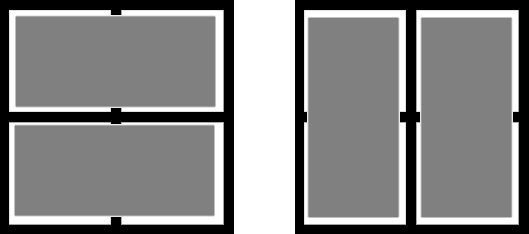
\includegraphics[width=0.4\textwidth]{images/domino_arrangements/2x2_all.png}
    \caption{all arrangments in a $2 \times 2$ grid.}
\end{figure}

\begin{figure}[H]
    \centering
    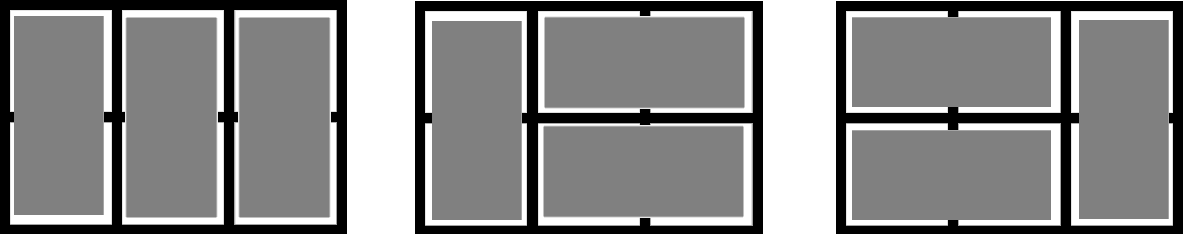
\includegraphics[width=0.7\textwidth]{images/domino_arrangements/2x3_all.png}
    \caption{all arrangments in a $2 \times 3$ grid.}
\end{figure}

\begin{figure}[H]
    \centering
    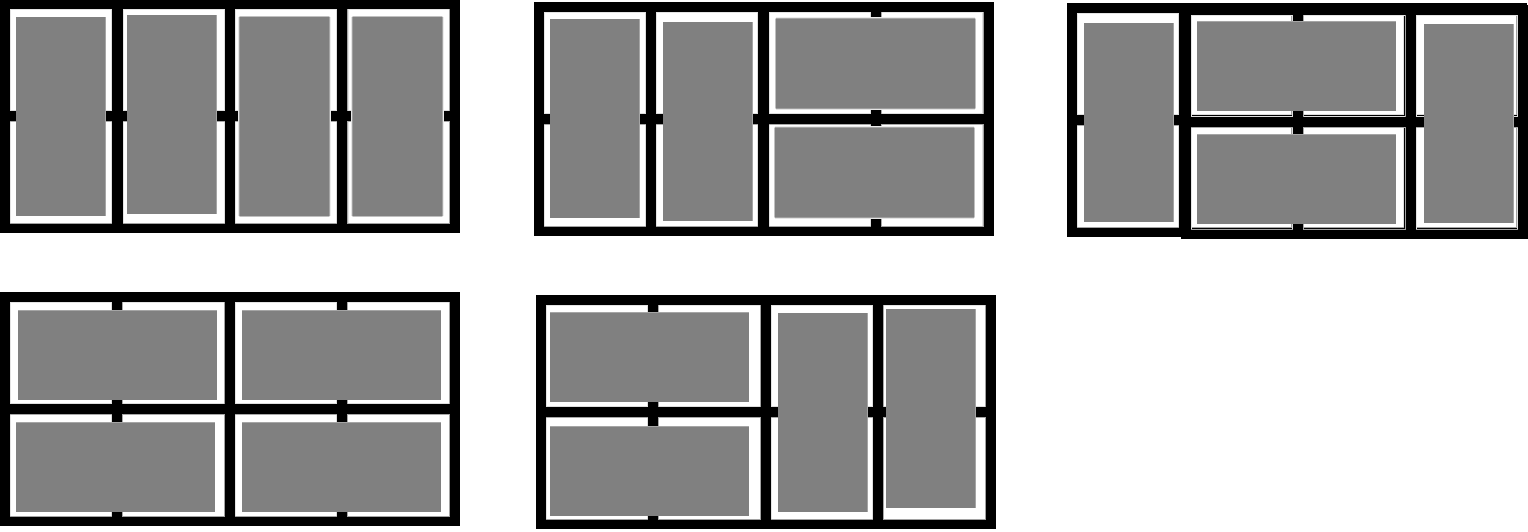
\includegraphics[width=0.9\textwidth]{images/domino_arrangements/2x4_all.png}
    \caption{all arrangments in a $2 \times 4$ grid.}
\end{figure}

\section{Algorithm}

Given $n \in \N$, let $S(n)$ be the solution (all arrangements). $S(n)$ can be obtained from two recursive calls:
\begin{enumerate}
    \item one vertical domino combined with $S(n-1)$;
    \item two horizontal dominos combined with $S(n-2)$;
\end{enumerate}
Such procedure is shown in the Figure

\begin{figure}[H]
    \centering
    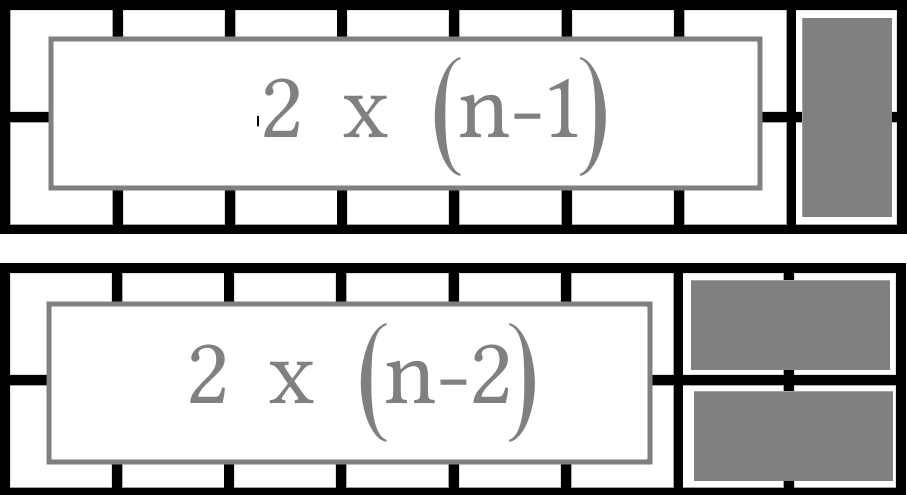
\includegraphics[width=0.7\textwidth]{images/domino_arrangements/2xn_recursive.png}
    \caption{recursive solution for a $2 \times n$ grid.}
\end{figure}

\section{Algorithm}

\begin{figure}[H]
    \centering
    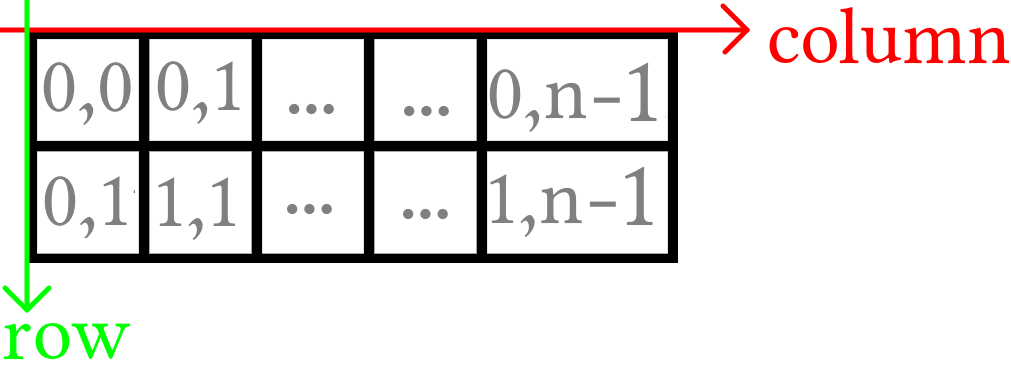
\includegraphics[width=0.9\textwidth]{images/domino_arrangements/grid_cordinates.png}
    \caption{coordinate system for a $2 \times n$ grid.}
\end{figure}

\newcommand{\domino}[2]{\mbox{\textbf{Domino}}\left[\tuple{#1}, vertical\right]}
\newcommand{\dominoV}[1]{\domino{#1}{vertical}}
\newcommand{\dominoH}[1]{\domino{#1}{horizontal}}
\newcommand{\DA}{domino\_arrangements}

\begin{algorithm}[H]
    \caption{\DA}
    \label{domino-arrangements:algorithm}
    \begin{algorithmic}[1]
        \Require{$n \in \N$}
        \If{$n == 1$}
            \State{\textbf{return} $$\Big\langle
                    \tuple{\dominoV{0,0}}
                \Big\rangle$$
            }
            \label{domino-arrangements:algorithm:n=1}
        \ElsIf{$n == 2$}
        \State{\textbf{return} $$\Big\langle
                \tuple{\dominoV{0,0}, \dominoV{0,1}},
            $$$$
                \tuple{\dominoH{0,0}, \dominoH{1,0}}
            \Big\rangle$$
            \label{domino-arrangements:algorithm:n=2}
        }
        \Else
            \State{\textbf{return} $$
                \text{\DA}(n-1) \oplus \tuple{\dominoV{0,0}},
                $$$$
                \text{\DA}(n-2) \oplus \tuple{\dominoH{0,0}, \dominoH{1,0}}
            $$}
            \Comment{$\oplus$ is the concatenation of the list on the right with all the lists on the left.}
        \EndIf
    \end{algorithmic}
\end{algorithm}

\section{Correctness of the Algorithm}

\subsection*{Base Case 1}

By inspection, one notices that for a $2 \times n$ grid, there are two possible arrangements. Therefore, the line \ref{domino-arrangements:algorithm:n=1} of the algorithm returns the optimal solution of the case $n = 1$.

\subsection*{Base Case 2}

By inspection, one notices that for a $2 \times n$ grid, there are two possible arrangements. Therefore, the line \ref{domino-arrangements:algorithm:n=2} of the algorithm returns the optimal solution of the case $n = 2$.

\subsection*{Recursion}

First of all, notice that, if a domino is in the horizontal position, then there must be a domino right over (or below) it. In other words, arrangements such as the one of the Figure \ref{domino-arrangements:figure:impossible-arrangement}.

Now, for the last domino, there is two possibilities: either it is in the vertical or the horizontal (and so there is another one below it) position. But for both cases, the problem of arranging the other dominos is the same problem but with a smaller grid:

\begin{enumerate}
    \item the last domino is in the vertical position: solve the problem for the grid $2 \times (n-1)$
    \item the last domino is in the horizontal position: solve the problem for the grid $2 \times (n-2)$
\end{enumerate}

\begin{figure}[H]
    \centering
    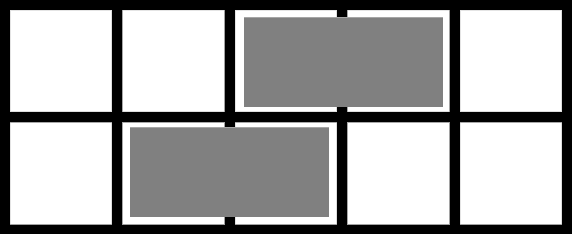
\includegraphics[width=0.6\textwidth]{images/domino_arrangements/2x5_impossible.png}
    \caption{invalid configuration of dominos. A horizontal domino must have another right over or below it.}
    \label{domino-arrangements:figure:impossible-arrangement}
\end{figure}


\end{document}
